\newpage
\chapter{Reconstrução de uma câmera $P$: Kuang e {\AA}str{\"o}m}\label{sec.astrom}

Nesta seção apresentaremos o problema da determinação da pose de uma câmera, que tem sido estudado extensivamente pela comunidade da área de visão computacional. Por exemplo, o caso mínimo da determinação da pose de uma câmera usando três pontos foi estudado inicialmente por Fischler e Bolles (1981) e outras formulações para problemas mínimos desse tipo foram comparadas e revisadas por N\"ole et al. (1994). Usando retas, foi desenvolvida uma solução mínima com três retas e suas correspondências por Chen (1991), e outro desenvolvimento envolvendo retas pode ser encontrado em Dhome et al. (1989). Recentemente, um caso mínimo usando combinação de pontos e retas foi publicado por Ramalingam et al. (2011). E mais recentemente ainda, visando aplicação em correspondência entre curvas Fabbri et al. (2012) desenvolveram uma solução mínima usando dois pontos-tangentes (definidos mais a frente).

Uma câmera pode ser fatorada em $P=K[R|{\bf t}]$, e o artigo de Kuang e \AA str\"om (2013) trata da determinação dos parâmetros externos $R$ e ${\bf t}$, considerando que são conhecidos quase todos os parâmetros internos da matriz $K$, menos a distância focal $f$. Assim, o artigo busca determinar sete parâmetros no total, três na matriz de rotação $R$, três no vetor de translação ${\bf t}$ e um na matriz de calibração. Alguns trabalhos anteriores já resolveram problemas de determinação desses sete parâmetros mas todos eles usaram somente correspondência entre pontos 3D e pontos 2D, $\X\leftrightarrow\x$, e as principais contribuições do artigo são o uso de correspondências entre outras entidades geométricas como retas e pontos-tangentes, e a apresentação de um procedimento para resolução de sistemas de equações polinomiais utilizando as bases de Gr\"obner e a matriz de ação. Temos interesse nessa tecnologia computacional para o trabalho futuro de auto-calibração trifocal usando curvas e superfícies. 

Como já vimos, os parâmetros externos $R$ e ${\bf t}$ tem a finalidade de trazer um ponto 3D escrito no sistema de coordenadas do mundo para o sistema de coordenadas da câmera, e na Figura \ref{fig.camera-astrom} podemos observar a ação de $[R|{\bf t}]$ bem como a correspondência entre entidades geométricas.
\begin{figure}[!htb]{.8\textwidth}
\caption{Projeç\~ao de retas, pontos e tangentes.}
\includegraphics[width=\hsize]{camera-astrom}
\source{Kuang e \AA strom (2013).}
\label{fig.camera-astrom}
\end{figure}
\section{Formulação do problema}

O artigo utiliza o modelo {\it pinhole} de câmera para aplicar a projeção de um ponto $\X$ em 3D em sua imagem $\x$ em 2D dada pela equação de projeção
\begin{equation}\label{eq.projecao}
\lambda\,\x=P\,\X,
\end{equation}
onde a matriz $P_{3\times4}$ pode ser fatorada conforme descrito acima, e $\lambda$ é um fator de escala descrito na Subseção \ref{sec.ponto}. 

Para obter estabilidade numérica e uma configuração prática da câmera, geralmente se assume que o plano da imagem tem o ponto principal centrado na origem, pixels quadrados e eixos perpendiculares ({\it skew} zero). Como a única incógnita na matriz de calibração é a distância focal, a mesma pode ser descrita como
\begin{equation}\label{eq.astrom-K}
K=
\begin{bmatrix}
1&0&0\\
0&1&0\\
0&0&w
\end{bmatrix},
\end{equation}
onde $w=\frac{1}{f}$.
\section*{Quantidade de equações.}

Cada objeto geométrico nos fornece uma determinada quantidade de equações para determinarmos os parâmetros de $P$, e vamos analisar de que forma esses objetos providenciam tais equações. Na Figura \ref{fig.astrom-objetos-geo} podemos visualizar um exemplo de cada uma das entidades geométricas.
\begin{figure}[!htb]{\textwidth}
\caption{Objetos geom\'etricos.}
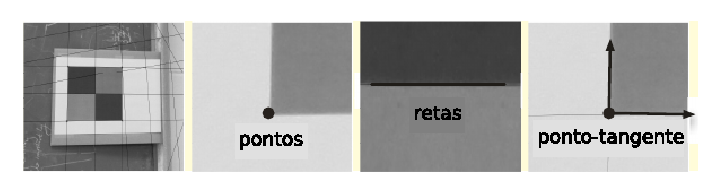
\includegraphics[width=\hsize]{astrom-objetos-geo}
\legend{Objetos utilizados para gerar equações na determinação dos parâmetros de $P$.}
\source{Kuang e \AA strom (2013).}
\label{fig.astrom-objetos-geo}
\end{figure}
\section*{Equações obtidas usando pontos.}

Dado um ponto 3D $\X$ e sua respectiva imagem em 2D $\x=(x,y,1)^\top$, a equação de projeção $\lambda\,\x=P\,\X$ nos fornece três equações. Mas, pela Subseção \ref{sec.ponto}, um ponto 2D tem apenas dois graus de liberdade apesar de suas três componentes, então dessas três equações apenas duas são linearmente independentes. Para eliminarmos o fator de escala $\lambda$ aplicamos o produto vetorial em ambos os lados da equação de projeção:
\begin{equation}\label{eq.astrom-pontos}
\begin{array}{rcl}
\lambda\,\x&=&P\,\X\\
\lambda\,[\x]_\times\x&=&[\x]_\times P\,\X\\
{\bf 0}&=&[\x]_\times P\,\X.
\end{array}
\end{equation}
\section*{Equações obtidas usando retas.} 

Uma reta 3D ${\bf L}$ pode ser representada usando um ponto $\X$ e uma direção ${\bf D}$, na forma ${\bf L}=\X+k\,{\bf D}$. Dadas a reta ${\bf L}$ e sua imagem $\lightrgb$ obtemos duas equações usando os dois pontos $\X$ e ${\bf D}$. Um ponto $\x$ pertence a uma reta $\lightrgb$ se $\lightrgb^\top\x=0$, e substituindo essa relação na equação de projeção \ref{eq.projecao} temos:
\begin{equation}\label{eq.astrom-retas}
\begin{array}{rcll}
\lightrgb^\top P\,\X&=&0&\text{se}\,\,\,k=0\\
\lightrgb^\top P(\X+k\,{\bf D})&=&0&\text{se}\,\,\,k\neq0.
\end{array}
\end{equation}  
\section*{Equações obtidas usando pontos-tangentes.}

É possível obter mais três equações se conhecemos o ponto $\X$, uma direção ${\bf D}$ através $\X$ bem como suas respectivas imagens $\x$ e ${\bf d}$. Com a correspondência $\X\leftrightarrow\x$ podemos usar a relação apresentada na Equaç\~ao \ref{eq.astrom-pontos} e conseguir duas equações. Para a terceira equação, usamos a reta definida pelos pontos na imagem, $\lightrgb=\x\times{\bf d}$, juntamente com as Equações \ref{eq.astrom-retas}, pois tomando a diferença entre tais equações e usando a reta $\lightrgb$ temos
\begin{equation}\label{eq.astrom-direcao}
\lightrgb^\top P\,{\bf D}=0.
\end{equation}  
Note que essas três equações são obtidas usando um ponto-tangente com uma direção apenas. Se usarmos ponto-tangente com mais direções, conseguimos uma equação a mais para cada direção, pois para cada ${\bf D}_i$ das $n$ direções, teremos $\lightrgb_i=\x\times{\bf d}_i$ e podemos formular as equações
\begin{equation}
[\x]_\times P\,\X={\bf 0}\quad\text{e}\quad\lightrgb_i^\top P\,{\bf D}_i=0\quad\text{para}\,\,i=1,...,n.
\end{equation}
Na tabela abaixo podemos verificar um resumo da quantidade de equações conseguidas para correspondências entre cada objeto geométrico.
\begin{center}
\begin{tabular}{|c|c|c|c|}
\hline 
{\bf ponto} & {\bf reta} & {\bf ponto com 1 tangente} & {\bf ponto com 2 tangentes} \\ 
\hline 
2 & 2 & 3 & 4 \\ 
\hline 
\end{tabular} 
\end{center}
\section*{Casos úteis.}

Com as quantidades de equações fornecidas por cada correspondência podemos formar várias combinações entre pontos, retas e ponto-tangentes para obtermos as sete equações necessárias para calcular os sete graus de liberdade de $P$. Vamos ver dois exemplos de problema mínimo.
\begin{itemize}
\item {\bf Dois pontos e um ponto-tangente (P2T1)}: com essa combinação temos três pontos e uma direção passando por um dos pontos, então podemos formar seis equações usando a Relação \ref{eq.astrom-pontos} e mais uma equação usando a Relação \ref{eq.astrom-direcao}. 

\item {\bf Um ponto-tangente com uma direção mais um ponto-tangente com duas direções (T1T2)}: temos uma reta passando por um dos pontos e duas retas passando pelo outro ponto, então podemos formar quatro equações usando \ref{eq.astrom-pontos} e mais três equações usando \ref{eq.astrom-direcao}.
\end{itemize} 

Podemos formar outros problemas mínimos conforme os apresentados aqui e vamos mostrar agora um caso supra-restringido, onde temos mais equações do que incógnitas a determinar.
\begin{itemize}
\item {\bf Quatro retas (P4L)}: Dadas quatro correspondências entre retas temos oito equações usando as Relações \ref{eq.astrom-retas}. Como precisamos de sete equações podemos usar uma delas para verificar a solução dada pelas demais.
\end{itemize}
\section*{Parametrização de $P$.}

Uma das ideias teóricas mais importantes do método e que a matriz de rotação da câmera é parametrizada com quaternions, pois desse modo produz sistemas de equações polinomiais relativamente fáceis de serem resolvidos. Utilizando quaternions, a matriz de rotação é dada por
\begin{equation*}
R=
\begin{bmatrix}
a^2+b^2-c^2-d^2&2bc-2ad&2ac+2bd\\
2ad+2bc&a^2-b^2+c^2-d^2&2cd-2ab\\
2bd-2ac&2ab+2cd&a^2-b^2-c^2+d^2
\end{bmatrix}
\end{equation*}
Se tratando de uma representação em coordenadas homogêneas podemos usar uma das variáveis para fixar a escala, assim tomando $a=1$ reduzimos o número de variáveis e facilitamos a solução do sistema de equações polinomiais.

O vetor de translação é parametrizado normalmente como ${\bf t}=(t_x,t_y,t_z)^\top$ e a matriz $[R|{\bf t}]$ se torna
\begin{equation*}
[R|{\bf t}]=
\begin{bmatrix}
a^2+b^2-c^2-d^2&2bc-2ad&2ac+2bd&t_x\\
2ad+2bc&a^2-b^2+c^2-d^2&2cd-2ab&t_y\\
2bd-2ac&2ab+2cd&a^2-b^2-c^2+d^2&t_z
\end{bmatrix}
\end{equation*}
Para completar a matriz $P$ basta aplicar, à esquerda de $[R|{\bf t}]$ a matriz de calibração $K$ conforme \ref{eq.astrom-K}.
\begin{equation*}
\begin{array}{rcl}
P&=&K\,[R|{\bf t}]\\\\
&=&
\begin{bmatrix}
1&0&0\\
0&1&0\\
0&0&w
\end{bmatrix}
\begin{bmatrix}
a^2+b^2-c^2-d^2&2bc-2ad&2ac+2bd&t_x\\
2ad+2bc&a^2-b^2+c^2-d^2&2cd-2ab&t_y\\
2bd-2ac&2ab+2cd&a^2-b^2-c^2+d^2&t_z
\end{bmatrix}\\\\
&=&
\begin{bmatrix}
a^2+b^2-c^2-d^2&2bc-2ad&2ac+2bd&t_x\\
2ad+2bc&a^2-b^2+c^2-d^2&2cd-2ab&t_y\\
w\,(2bd-2ac)&w\,(2ab+2cd)&w\,(a^2-b^2-c^2+d^2)&w\,t_z
\end{bmatrix}
\end{array}
\end{equation*} 
Substituindo $t'_z=w\,t_z$, temos que determinar as sete variáveis $\{b,c,d,t_x,t_y,t'_z,w\}$. Mas observe que as variáveis $\{t_x,t_y,t'_z\}$ são todas lineares usando as Relações \ref{eq.astrom-pontos}, \ref{eq.astrom-retas} e \ref{eq.astrom-direcao}, e portanto podem ser eliminadas do sistemas de equações restando apenas as quatro variáveis $\{b,c,d,w\}$. Depois de determinadas essas quatro variáveis, o vetor de translação pode ser recuperado por substituição. 
\section{Sistema de equações polinomiais}

Para resolver computacionalmente os sistemas de equações polinomiais decorrentes do emprego dos casos úteis na determinação de $P$, Kuang e \AA str\:om (2013) utilizam m\'etodos baseados em geometria algébrica. Primeiramente, utilizando a ferramenta {\it Macaulay2}, Grayson e Stillman (1993-2002), é verificada a existência de 20 soluções para o caso mínimo (P2T1). Para sistemas com pouca quantidade de variáveis, usar apenas o método das bases de Gr\"obner pode ser rápido e numericamente estável, mas aqui é empregado o método exposto em Byr\"od et al. (2009), que consiste basicamente em extrair a base linear a partir das bases de Gr\"obner e empregar a matriz de ação, da qual as soluções podem ser obtidas pela decomposição em autovalores. No apêndice \ref{sec.geo-algebrica} é fornecido um resumo sobre a teoria básica de geometria algébrica, bem como exemplos da utilização do método das bases de Gr\"obner e da matriz de ação para resolver sistemas computacionalmente.
